\begin{appendix}

\phantomsection \addcontentsline{toc}{chapter}{Anhang}

\chapter{Schaltplan und Layout des Mess-Clients}
\label{anhang_Schaltung}





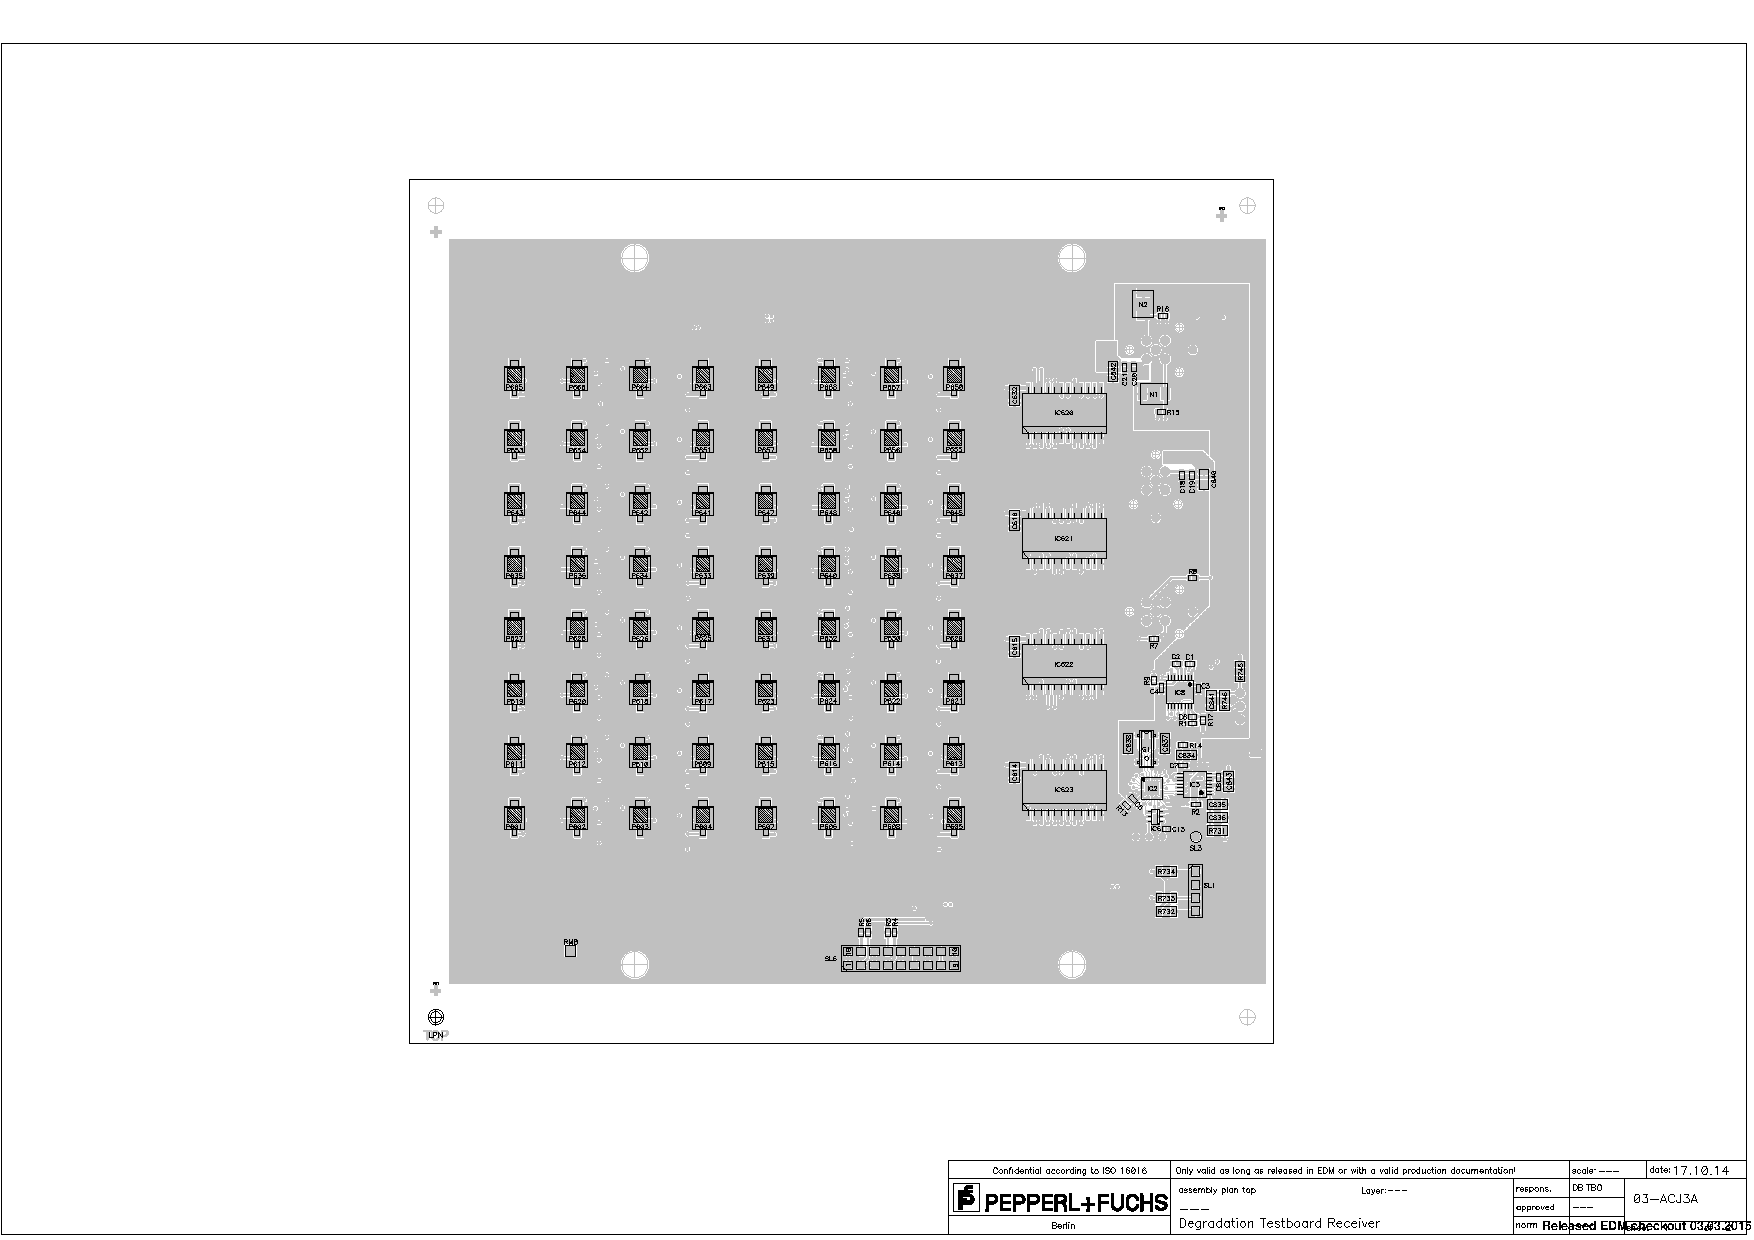
\includepdf[landscape=true,pages={1-2}]{Design.pdf}

\newpage

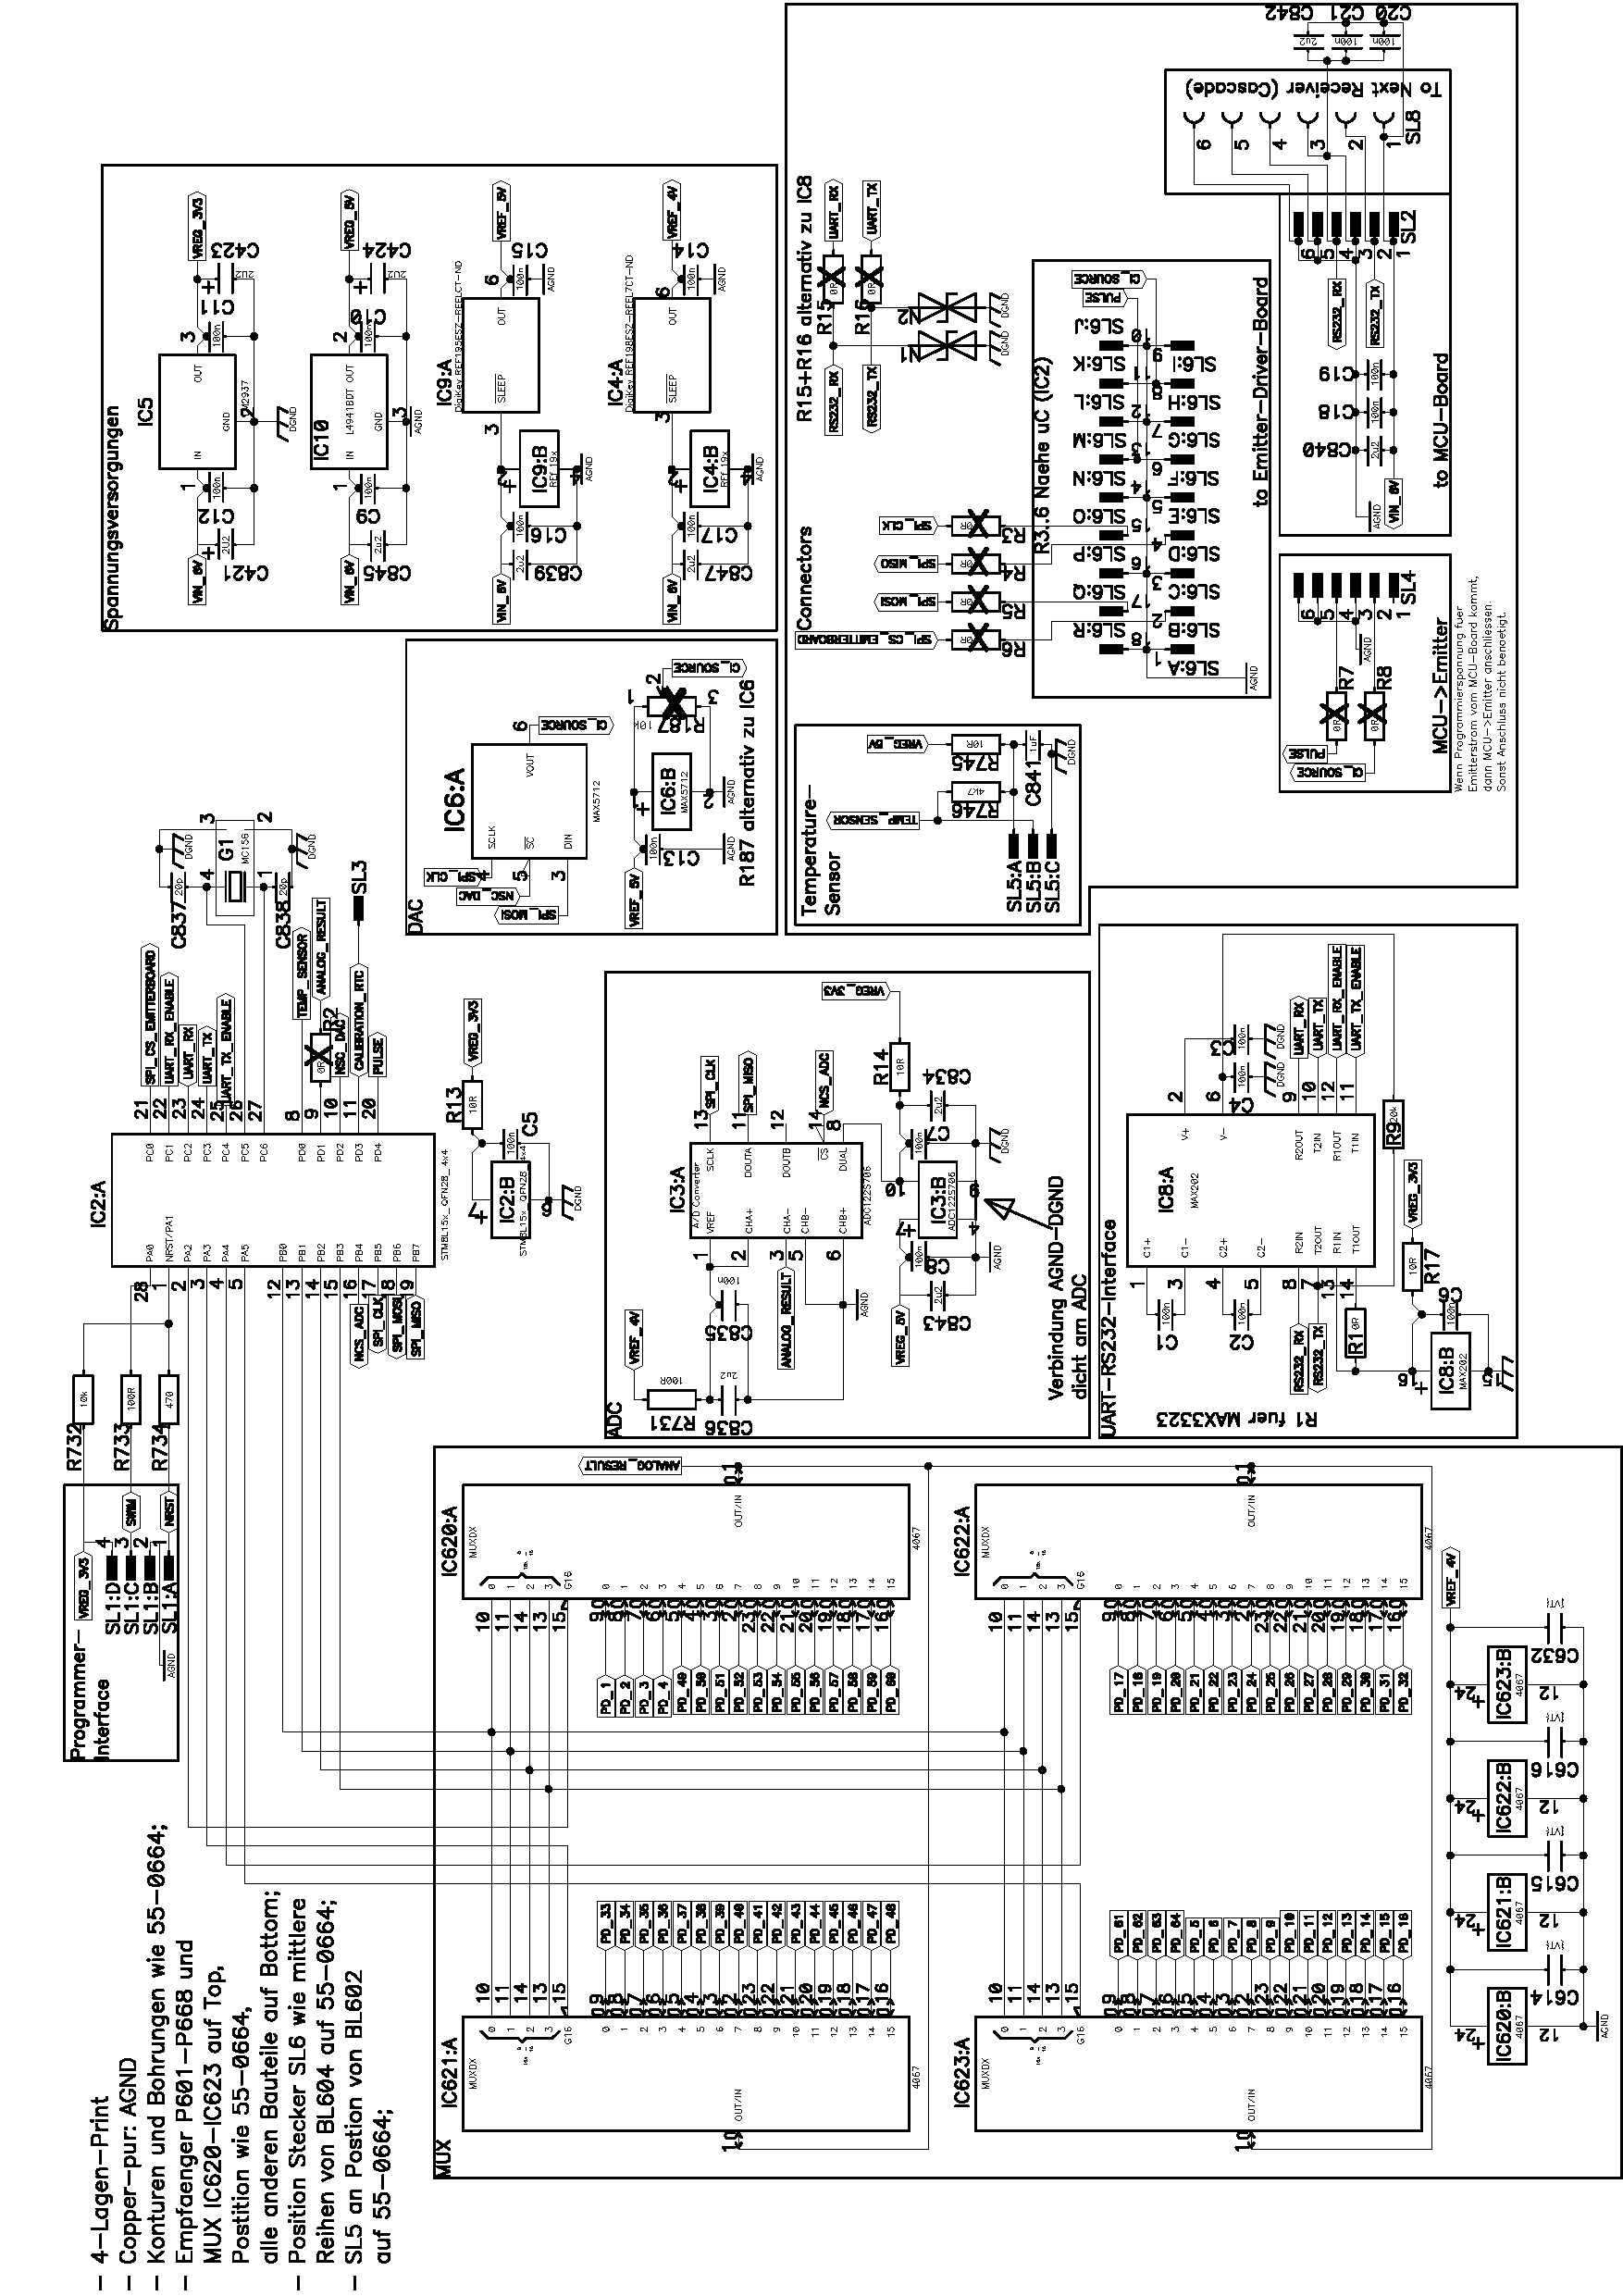
\includepdf[pages={1}]{Schaltung.pdf}
\chapter{Inhalt der beigefügten CD-ROM}
\label{anhang_cd}

\begin{table}[H]
\begin{center}
\begin{tabularx}{\textwidth}{ll}
 Thesis Tim Nieter.pdf & Diese Arbeit als PDF Dokument  \\
 Hardware/ & Enthält die Schaltungen und Layouts \\
 Quellcode/Datenbank & Quellcode zum erzeugen der Datenbank \\
 Quellcode/Mess-Client & Quellcode des Mess-Clients \\
 Quellcode/Mess-Server & Quellcode des Mess-Servers \\
 Quellcode/PC-Client & Quellcode des PC-Clients \\
 Tools/ & Bei der Entwicklung verwendete Werkzeuge

\end{tabularx}

\label{table_CD}
\end{center}
\end{table}

\end{appendix}
